\documentclass[aps,pre,preprint,groupedaddress]{revtex4-1}
\bibliographystyle{apsrev4-1}

\usepackage[pdftex]{graphicx}
\usepackage{amsmath}
\newcommand{\e}[1]{\cdot10^{#1}}
\let\endtitlepage\relax

\begin{document}

\title{Report HPC-Europa2 Transnational Access Programme}

\author{Oliver Henrich$^1$ and Kevin Stratford$^2$}

\affiliation{
$^1$Centre for Computational Science, University College London, United Kingdom\\
$^2$Edinburgh Parallel Computing Centre, University of Edinburgh, United Kingdom
}


\date{\today}
\begin{abstract}
This is the intermim report of our joint visit from 12 April - 11 May 2012 to Barcelona Supercomputing Center and Prof Ignacio Pagonabarraga, Departament de Fisica Fonamental, Universitat de Barcelona, Spain.
\end{abstract}


\maketitle

\section{Week 1 (including period 12-20 April)}

We have introduced an object to hold the scalar electric potential,
and the charge densities for a general number of species. This
includes specification of diffusivities, valencies and unit charge.
The corresponding parallel halo swaps and I/O routines have been
added and subjected to unit tests.

In discussions with Pagonabarraga, we decided to prioritise the
implemenation of the the Poisson solver (successive overrelaxation,
SOR) so that more simple validation problems can be attempted as
soon as possible. The SOR solver has been implemented and tested
against an exact matrix solver for a one-dimensional problem in
both serial and parallel. The SOR solver assumes a spatially
uniform permittivity. We will extend this to a spatially varying
permittivity at a later stage.

A start has been made on the finite difference solution of the
Nernst Planck equation (advection/diffusion equation for charged
species). This will be completed and tested next week. This puts
us slightly ahead of schedule cf the original work plan.

Basic tests of the SOR solver have been already performed.
We have identified a number of other suitable test scenarios to 
verify the implemention of the Nernst-Planck equation in 
combination with the SOR solver.
We decided to test the Gouy-Chapman theory
for electric double layers in front of a charged wall \cite{Lyklema},
the liquid junction potential emerging between two electrolytes
of slighty different concentration and diffusivity of the charged species \cite{Mafe},
electro-osmotic flow in a slit pore  
\cite{Capuani, Rotenberg} and Debye-H\"uckel theory for charged 
colloidal particles and small enough potentials \cite{Lyklema}.

\section{Week 2 (23-27 April)}

We completed the numerical implementation of the Nernst-Planck
Equation which is solved via a simple finite difference method.
The solution includes advection (although there is no fluid
fluid fluid present in the test problems). We have included
no normal flux boundary conditions at solid fluid interfaces
to ensure the conservation of charged species. The solver
has been tested in both serial and in parallel.

A first validation test is a flat surface carrying a surface charge $\sigma$
with counterions and symmetic electrolyte. This is a one-dimensional, 
electroneutral problem of a diffusive electric double layer which has 
an analytical solution \cite{Lyklema}. 
The approximation for low electrostatic 
potentials reads

\begin{equation}\label{gouychapman}
\Psi(x) = \Psi_D \exp(-\kappa\, x)
\end{equation}
with $\kappa$ as inverse Debye length 
\begin{equation}
\kappa = l_D^{-1} = \sqrt{8\pi\, l_B \, I}.
\end{equation}
The Bjerrum length $l_B$ is given by 
\begin{equation}
l_B = \frac{\beta\,e^2}{4\pi\,\varepsilon}
\end{equation} 

with $\beta^{-1}=k_B T$, $e$ as unit charge and $\varepsilon=\varepsilon_0\varepsilon_r$ 
as dielectric permittivity.
The parameter 

\begin{equation}
I = \frac{1}{2}\sum_k z_k^2\; \rho_{B,k}
\end{equation} 

is the ionic strength 
of the electrolyte with $z_k$ as valencies of species $k$
($z_\pm=\pm 1$ for simple symmetric electrolyte) and $\rho_{B,k}$ as 
bulk charge density of species $k$ far away from the wall.
The Stern potential $\Psi_D$ at the surface of the wall is related 
to the surface charge $\sigma$ via

\begin{eqnarray}
\Psi_D&=&\frac{2}{\beta \,e} \sinh^{-1}\left(-\sigma\,p\right)\\
\Psi_D&\simeq&\frac{2}{\beta \,e} \ln\left(-\sigma \, p + \sqrt{(\sigma\,p)^2+1}\right)\\
p &=& \frac{1}{\sqrt{8\, \varepsilon\, \beta^{-1} \,\rho_B}}.
\end{eqnarray}

The quantity $\rho_B=\rho_{B,+}=\rho_{B,-}$ is 
the average bulk charge density of the electrolyte.

We solved the Gouy-Chapman problem for a 
system consisting of $L_x \times L_y \times L_z=64\times4\times4$
lattice sites. Periodic boundary conditions were used at all sides 
and a no-flux boundary conditions was set at $L_x=1$ and $L_x=64$.
 
The parameters were chosen as follows (all in simulation units):
unit charge $e=1$, temperature $k_B T=\beta^{-1}=3.333\e{-5}$, valency $z_{\pm}=\pm1$, 
dielectric permittivity $\varepsilon=3.3\e{3}$, diffusivities 
of the species $D_{\pm}=1\e{-2}$ and initial densities $\rho_{0,\pm}=1\e{-2}$.
The entire system was electro-neutral and had a Bjerrum length $l_B=0.723$.

At first we tested the linear case applying a small positive surface charge
$\sigma=3.125\e{-2}$, which led to bulk charge density $\rho_{B,+}=\rho_{B,-}=1.044\e{-2}$, 
Debye length $l_D=2.295$ and surface potential $\Psi_D=2.136\e{-5}$.
The potential was initialised with zero and had a value $\Psi_c=-2.364\e{-6}$ 
in the centre of the system after equilibration which we subtracted in the 
following analysis.

We reduced the initial density of the electrolyte to $\rho_{0,\pm}=1\e{-3}$,
which resulted in bulk charge densities  
$\rho_{B,+}=1.298\e{-3}, \rho_{B,-}=1.370\e{-3}$, 
Debye length $l_D=6.420$, surface potential $\Psi_D=5.451\e{-5}$
and centre potential $\Psi_c=-1.256\e{-5}$.
The comparison with the approximate solution Eq. \ref{gouychapman} is shown 
in Fig. \ref{fig1}.

\begin{figure}[h!t]
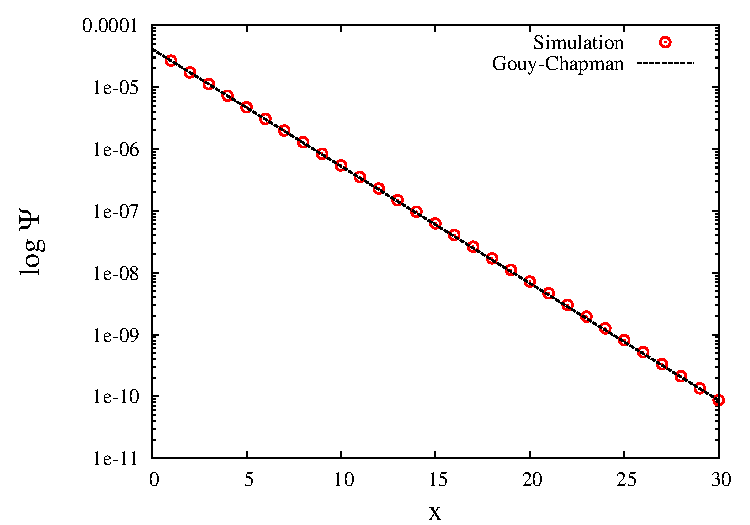
\includegraphics[width=0.495\textwidth]{test1.pdf}
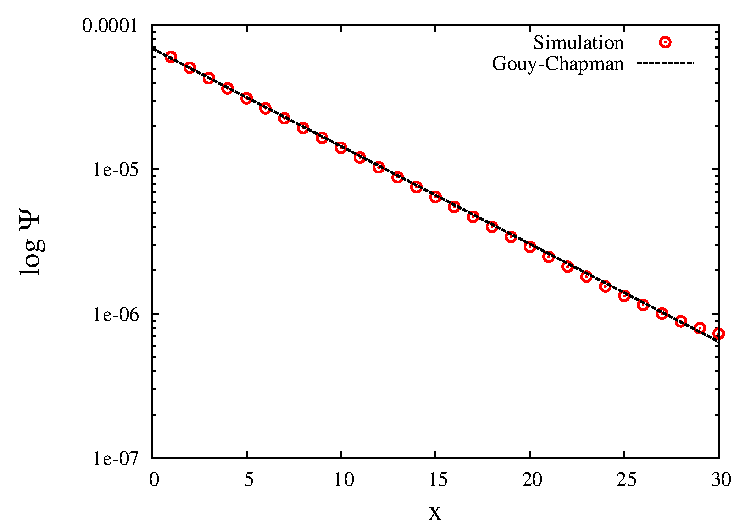
\includegraphics[width=0.495\textwidth]{test2.pdf}
\caption{Gouy-Chapman theory for electric double layers: The plots compare the simulation results for the electric potential with the analytical solution for $\rho_{0,\pm}=1\e{-2}$ (left) and $\rho_{0,\pm}=1\e{-3}$ (right).} 
\label{fig1} 
\end{figure}

For larger surface charges the low-potential assumption which led to Eq. \ref{gouychapman}
is no longer valid and the nonlinear nature of the Poisson-Boltzmann 
equation becomes evident.
Fig. \ref{fig2} shows the results for a surface charge $\sigma=9.375\e{-1}$
and electrolyte density $\rho_{0,\pm}=3\e{-3}$. We obtained for   
bulk charge densities $\rho_{B,+}=4.443\e{-3}$ and $\rho_{B,-}=4.461\e{-3}$, 
Debye length $l_D=3.514$, the surface potential $\Psi_D=2.267\e{-4}$
and the centre potential $\Psi_c=-3.395\e{-5}$. 

\begin{figure}[h!t]
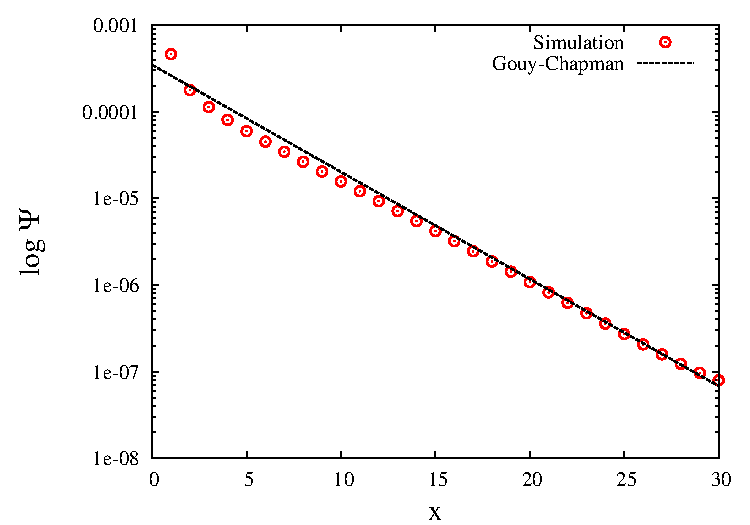
\includegraphics[width=0.495\textwidth]{test3.pdf}
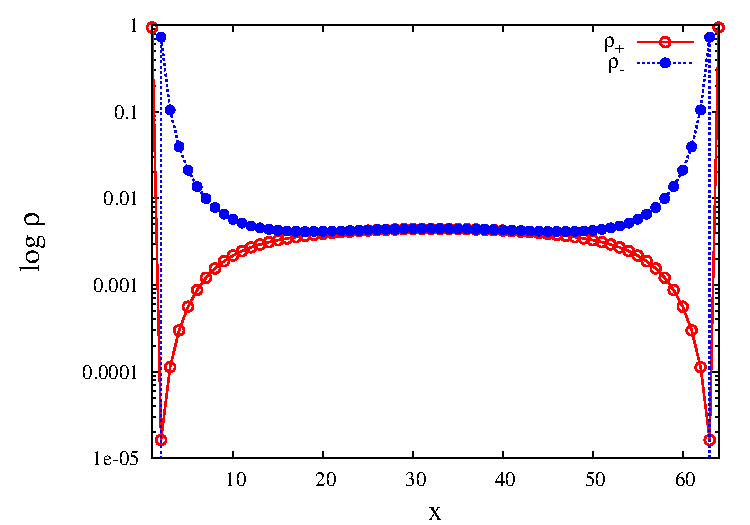
\includegraphics[width=0.495\textwidth]{test3-rho.pdf}
\caption{Nonlinear regime: For larger surface charges the solution deviates from the low-potential approximation Eq. \ref{gouychapman} to the Gouy-Chapman theory. The righthand picture shows the charge distribution across the gap.} 
\label{fig2} 
\end{figure}

A number of minor bugs in the parallel implementation of the
SOR solver were resolved, and the unit tests updated appropriately.

Some effort has been used to create a comprehensive test suite
for the basic functionality involved in these routines. These
tests are valid both in serial and in parallel.

Work is now under way to couple the new Nernst-Planck and
Poisson routines with the main code. This includes work to
include charged colloids.


\section{Week 3 (30 April - 4 May)}

We have now coupled the Poisson solver and the Nernst Planck solver
to the main code and checked for correct operation. This has included
the run time intialisation of the electrokinetic-related quatities
from the input file. We have also integrated the parallel I/O for
the electrokinetic lattice quantities to the main code, again with
appropriate initialisation from input.

We proceeded with another test. The liquid junction potential 
is a charge separation process that 
occurs when electrolytes with slightly different concentrations
whose species have different diffusivities are brought into contact.
Charges from the regions of higher concentration diffuse   
into the parts with lower concentration. Due to the difference 
in diffusivity they migrate at different speeds, leaving parts of
the system charged. This leads to a build-up of a potential
which balances the diffusive flux.

After the initial build-up phase the potential decreases slowly 
again until the charge concentration has become homogeneous throughout 
the system. Both timescales of emergence and decay of the potential
can be separated by chosing a sufficiently large system size.

This problem allowed us to verify the correct temporal 
behaviour of the Nernst-Planck equation solver by resolving the transient 
dynamics without having to account for advective terms.

For simplicity we considered systems of size 
$L_x\times L_y\times Lz=128\times4\times4$ and 
$L_x\times L_y\times Lz=256\times4\times4$ with
periodic boundary conditions at either end.
The two halfs were electroneutral and had ionic concentrations 
$\rho_{L,\pm}=\rho_{0,\pm} + \delta\rho$ and 
$\rho_{R,\pm}=\rho_{0,\pm} - \delta\rho$ 
with $\rho_{0,\pm}=1\e{-2}$ and $\delta\rho = 0.01$.

The potential difference between both sides during the build-up 
obeys approximately

\begin{equation}
\Delta\Psi(t)\simeq\Delta\Psi_P \left\{1-\exp\left(-\frac{t}{\tau_e}\right)\right\}\\
\end{equation}

with 

\begin{equation}
\Delta\Psi_P=\frac{(D_+ D_-)}{\beta e (D_+ + D_-)} \frac{\delta\rho}{\rho_0}\\ 
\end{equation}

as saturation value of the potential difference.
The saturation time scale is given by

\begin{equation}
\tau_e=\frac{\varepsilon}{\beta \, e^2 (D_+ + D_-) \rho_0}.
\end{equation}

A more exact solution can be derived in the limit $l_D/L_x<<1, N\to\infty$: 
 
\begin{eqnarray}
\Delta\Psi(t)&=&\Delta\Psi_P \left\{1-\exp\left(-\frac{t}{\tau_e}\right)\right\}\frac{4}{\pi}\left\{\sum_{m=1}^N \frac{\sin^3(m\pi/2)}{m} \exp\left(-\frac{ m^2\, t}{\tau_d}\right)\right\}\\
\tau_d&=&\frac{L^2}{2\pi^2 (D_+ + D_-)}.\label{taud}
\end{eqnarray}

It contains as well the dependence on the decay timescale $\tau_d$.
Only odd indices $m$ contribute to the sum:
 
\begin{eqnarray}
\sum_{m=1}^N \frac{\sin^3(m\pi/2)}{m} \exp\left(-\frac{m^2\, t}{\tau_d}\right)&=&\nonumber\\
&&\hspace*{-4cm} \exp\left(-\frac{t}{\tau_d}\right)-\frac{1}{3} \exp\left(-\frac{9 t}{\tau_d}\right)+\frac{1}{5}\exp\left(-\frac{25t}{\tau_d}\right)-\frac{1}{9}\exp\left(-\frac{81 t}{\tau_d}\right)+\ldots
\end{eqnarray}

A complete discussion of the solution can be found in \cite{Mafe}. 
There, the upper limit of significant modes has been also estimated as $N_{max} = L/\pi l_D$.
Note the factor 2 difference between Eq. \ref{taud} and the corresponding expression in \cite{Mafe}.
\begin{figure}[h!t]
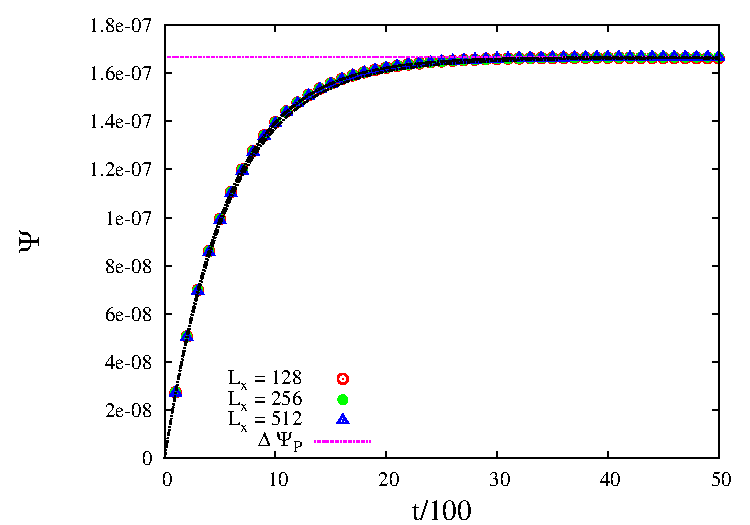
\includegraphics[width=0.495\textwidth]{test_lj_zoom1.pdf}
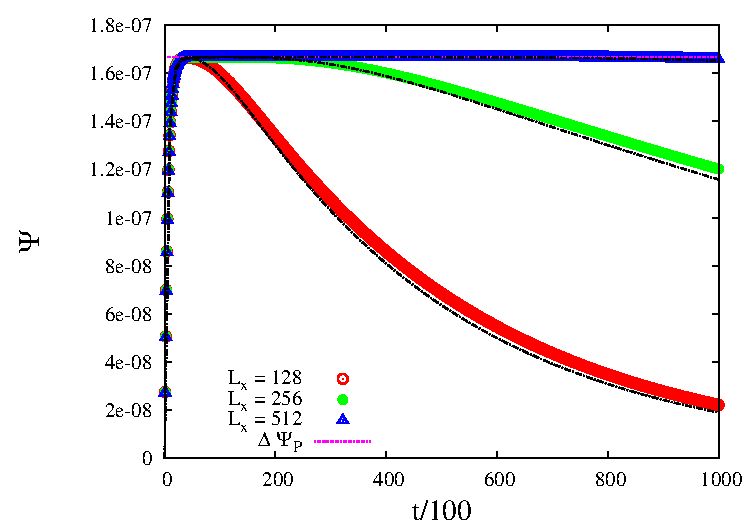
\includegraphics[width=0.495\textwidth]{test_lj_zoom3.pdf}
\caption{Time evolution of the liquid junction potential for $L_x=128$ (blue), $L_x=256$ (green) and $L_x=512$ (blue). The dashed black curves represent the approximate solution in the limit $l_D/L_x<<1$. Deviations can be seen which are due
to the finite size of our system and the approximate nature of the analytical solution.} 
\label{fig3} 
\end{figure}

The following parameters were used:
dielectric permittivity $\epsilon=3.3\e{3}$, temperature $\beta^{-1}=3.333\e{-5}$, unit charge $e=1$, valency $z_\pm=\pm1$, diffusivities $D_+=0.0125$ and $D_-=0.0075$.
We obtained
$\Delta\Psi_P=1.6667\e{-7}$, $\tau_e=550$, $\tau_d=41501.2\, (L_x=128)$, $\tau_d=166004.6\, (L_x=256)$ and $\tau_d=664018.5 (L_x=512)$.
The results for the potential difference over time are shown in Fig. \ref{fig3}.


\begin{figure}[h!t]
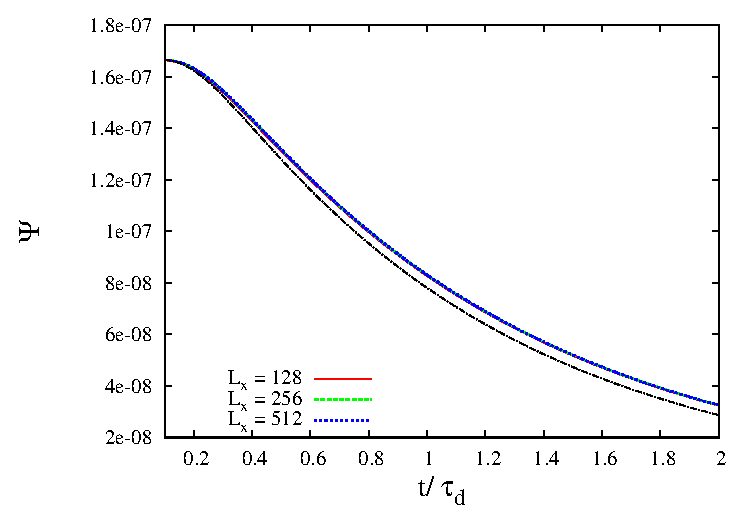
\includegraphics[width=0.9\textwidth]{test_lj_decay1.pdf}
\caption{Rescaled plot of the decay: Times have been Time evolution of the liquid junction potential for $L_x=128$ (blue), $L_x=256$ (green) and $L_x=512$ (blue). The dashed black curves represent the approximate solution in the limit $l_D/L_x<<1$. Deviations can be seen which are due
to the finite size of our system and the approximate nature of the analytical solution.} 
\label{fig4} 
\end{figure}

Fig. \ref{fig4} shows results with times rescaled to the decay 
time scale $\tau_d$ (cf. Eq. \ref{taud}). Obviously the 
deviations we observe are not due to the limited system size 
and have a more systematic origin. 

The curves coincide if 
the theoretic limit for $\tau_d$ is rescaled by a factor $1.067$,
suggesting the effective system length for this sort of setup is
actually about 3\% larger than the numerical value.

A reason for this might be that the analytical solution was gained
for an infinitely large system with constant charge concentrations,
vanishing currents at both ends and finite diffusive zone of size $L_x$.
In our situation the entire system is within the diffusive zone.
This may lead to smaller effective diffusivities or larger effective
system sizes.
Interestingly, all runs with solid walls at both ends resulted in 
oscillatory behaviour and an effective system size of $2L_x$.


We have run some simple scaling tests for the electrokinetic problem
with zero fluid velocity. A system of $128^3$ lattice sites was used
as representative of a small production system. The code was run on
the Mare Nostrum machine in Barcelona for a small number of time
steps to assess performance on up to 512 MPI tasks. The results are
shown in Fig. \ref{fig5}. 

While the scaling for the Nernst Planck part of
the calulcation are reasonable, it can be seen that the SOR routine
used to solve the Poisson equation is not really acceptable. This
was not unexpected. Some improvements might be possible, but the
algorithm is essentailly unsuitable for large systems. We will
investigate the use of an alternative (e.g., multigrid), but this
is beyond the scope of this HPC Europa visit.

In discussion with Pagonabarraga, we have also made some progress
in deciding how to modify a number of other parts of the code to
allow for the presence of the electric potential. These include
the free energy calculation, which can be generalised to compute
both electric contributions and coupling between potential and
compositional order parameter. A flexible solution may require
some refactoring.

We have also implemented a fixed external electric field in the
Nernst Planck equation. This will be tested during the last week
of the visit.

\begin{figure}[h!t]
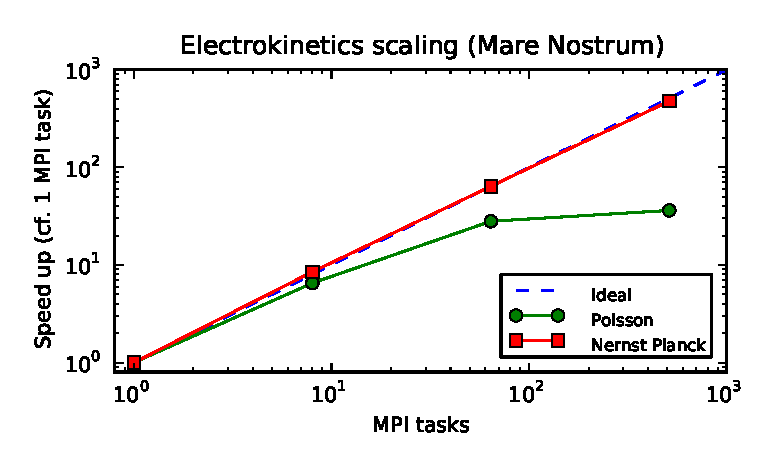
\includegraphics[width=0.9\textwidth]{scaling.pdf}
\caption{Scaling of a system of $128^3$ lattice sites on up to 512 MPI tasks. 
While the scaling for the Nernst Planck part of the calulcation are reasonable, 
it can be seen that the SOR routine used to solve the Poisson equation deviates
strongly from ideal behaviour.} 
\label{fig5} 
\end{figure}

\section{Week 4 (7 May - 11 May)}

To test the implementation with all couplings to external and 
internal forces we consider a forced charged fluid in a slit
of size $L_z$. An electrostatic field $E_{||}$ is allied
parallel to the walls. The entire system is electroneutral with 
each wall having the surface charge density $\sigma$ 
and compensationg counterions with total charge $2 \sigma A_{wall}$
in the fluid.

In equilibrium the charge density at a distance $x$ from the wall obeys

\begin{equation}
\rho(x)=\frac{\rho_0}{\cos^2(K\,x)}
\end{equation}

with 

\begin{equation}
\rho_0=K^2/2\pi l_B
\end{equation}

and 

\begin{eqnarray}
K \,L_x \tan\left(\frac{K\, L_x}{2}\right)&=&\pi\, l_B\, L_x\, 2\sigma\label{kex} \\
K \,L_x&\simeq&\sqrt{4\pi \,l_B\,L_x\,2\sigma}\label{klin}.
\end{eqnarray}

The liniarised version Eq. \ref{klin} has only a limited range of applicabilty.
We solved Eq. \ref{kex} numerically and found solutions 
$K=0.01959\; (\sigma=0.003125)$ and $K=0.03311\; (\sigma=0.00125)$, 
which is reasonably far away from the 
theoretical limit $K_{max}=\pi/L_x$ set by the tangent. 

Note the factor 2 difference on the lhs of Eq. \ref{kex} with respect 
to \cite{Capuani, Rotenberg}. There is also a factor $L_x$ missing on 
the rhs of Eq. \ref{klin}.

The steady state velocity of the fluid can be derived from the 
force balance of the gradient of the stresses and the electrostatic
forces:

\begin{eqnarray}
v_y(x)&=&\hat{v} \ln\left(\frac{\cos(K\,x)}{\cos(K\,L_x/2)}\right)\label{vy}\\
\hat{v}&=&\frac{e \,E_{||}\rho_o}{\eta\, K^2}=\frac{e \,E_{||}}{2\pi\eta l_B}\label{vhat}
\end{eqnarray}

The result for two different charge densities is shown in Fig. \ref{fig6}.
The accuracy is acceptable with deviations for high surface 
charged potentially being caused by the chosen discretisation or 
by the numerical solution of Eq. \ref{kex} approaching the limit 
of $\pi/L_z\simeq0.049$.  

\begin{figure}[h!t]
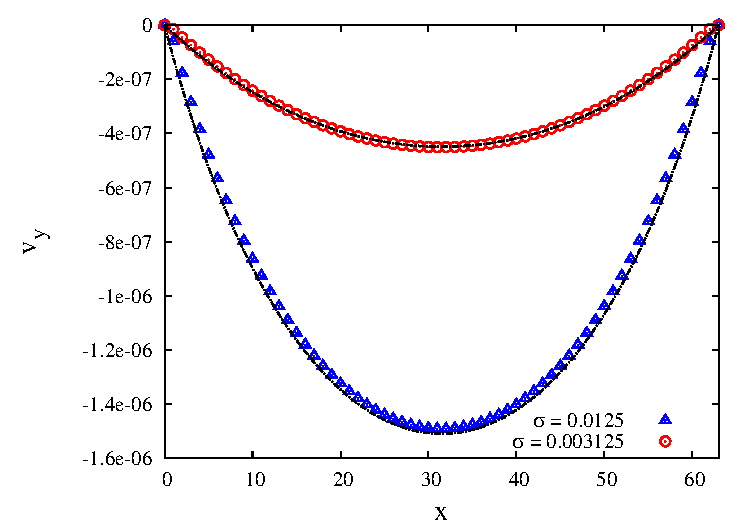
\includegraphics[width=0.9\textwidth]{test_eo.pdf}
\caption{Steady state flow profile across a slit of width $L_x=63$ for an applied field of magnitude $e \beta E L_x=1.89$ for two different charge densities $\sigma=0.003125$ (red) and $\sigma=0.0125$ (blue), Bjerrum length $l_B=0.7234$, viscosity $\eta=0.1$ and unit charge $e=1$. The dashed black lines correspond to theoretical prediction according to Eqs. \ref{vy} and \ref{vhat}.} 
\label{fig6} 
\end{figure}

Finally, we have tested the implementation for a single fixed
colloid and compared the result with Debye-H\"uckel theory. A result
is shown in Fig.~\ref{fig7}.
We used the following parametrisation:

$L_x \times L_y \times L_z=64\times64\times64$,
$D_+=D_-=0.01$,
$e=1$, 
$z_{\pm}=1$,
$\beta^{-1}=3.333\e{-5}$,
$\varepsilon=3.3\e{3}$,
$l_B=0.723$.

For a central and fixed colloid of radius $R_c=7.5$ carrying a positive unit charge
$q_{c,+}=1.0, q_{c,-}=0$ we obtained 
$\rho_{c,+}=5.58\e{-4}$,
$\rho_{el}=\rho_{B,\pm}=1\e{-2}$, 
$\Psi_D=8.836\e{-7}$ for $2\,R_c=16$.

For a higher larger positive charge $q_{c,+}=4.0$ we got
$\rho_{c,+}=2.23\e{-3}$
$\rho_{el}=\rho_{B,\pm}=5\e{-3}$ 
$\Psi_D=4.993\e{-6}$ for $2\,R_c=16$.

\begin{figure}[h!t]
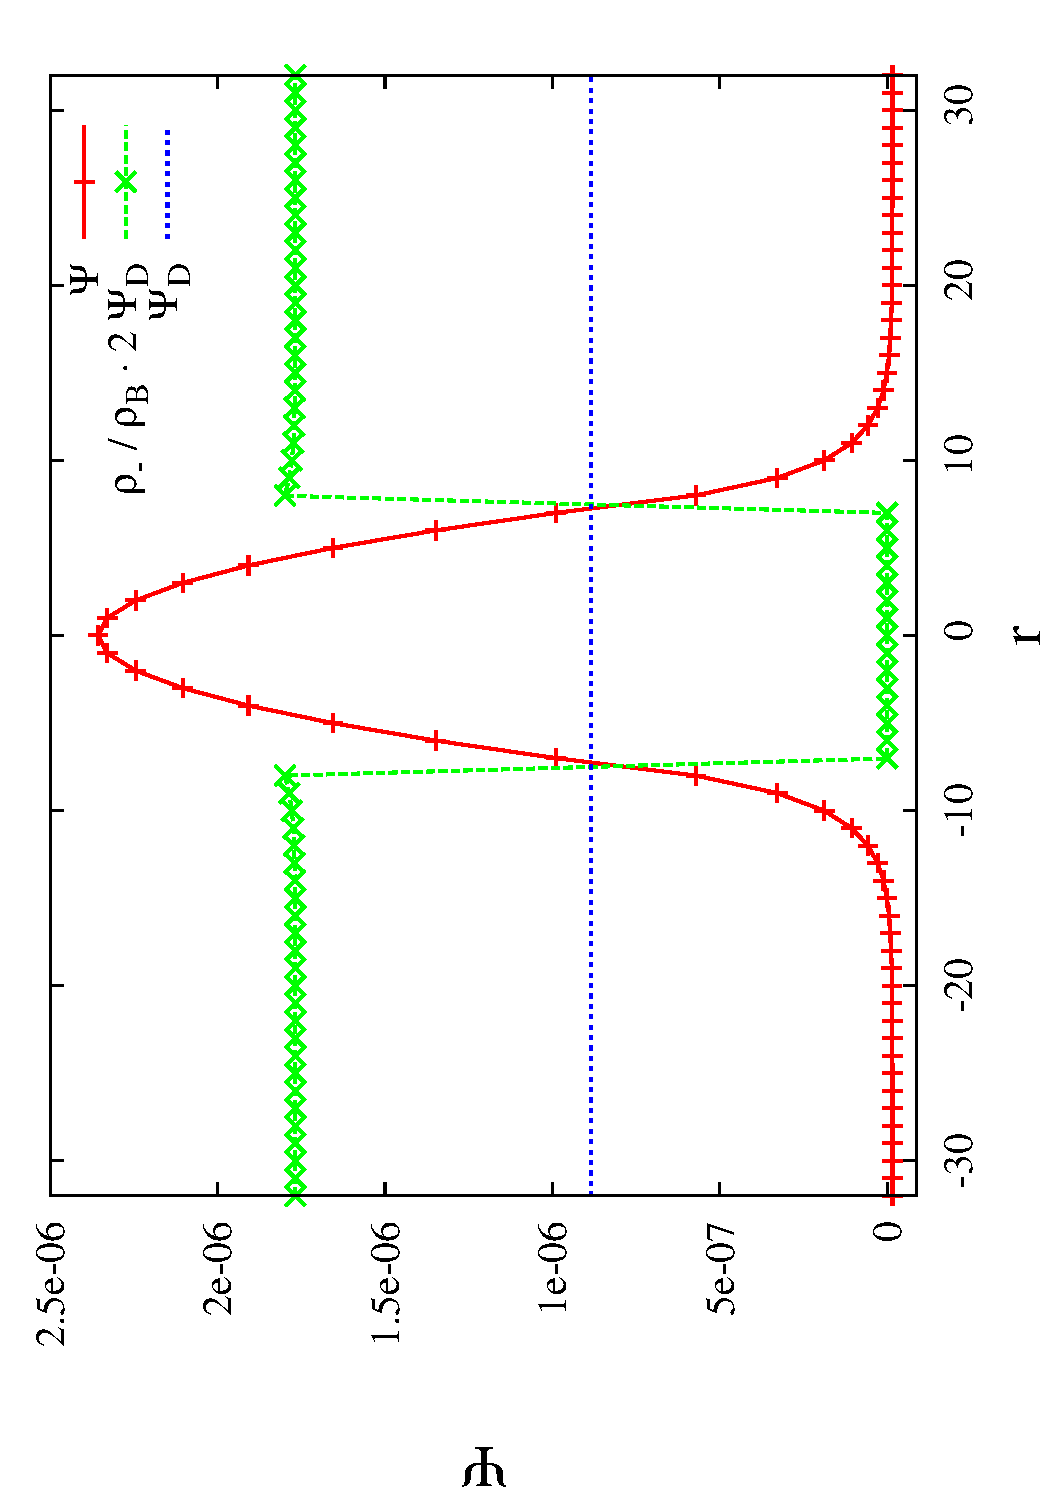
\includegraphics[angle=-90,width=0.9\textwidth]{test_dh1.pdf}\\
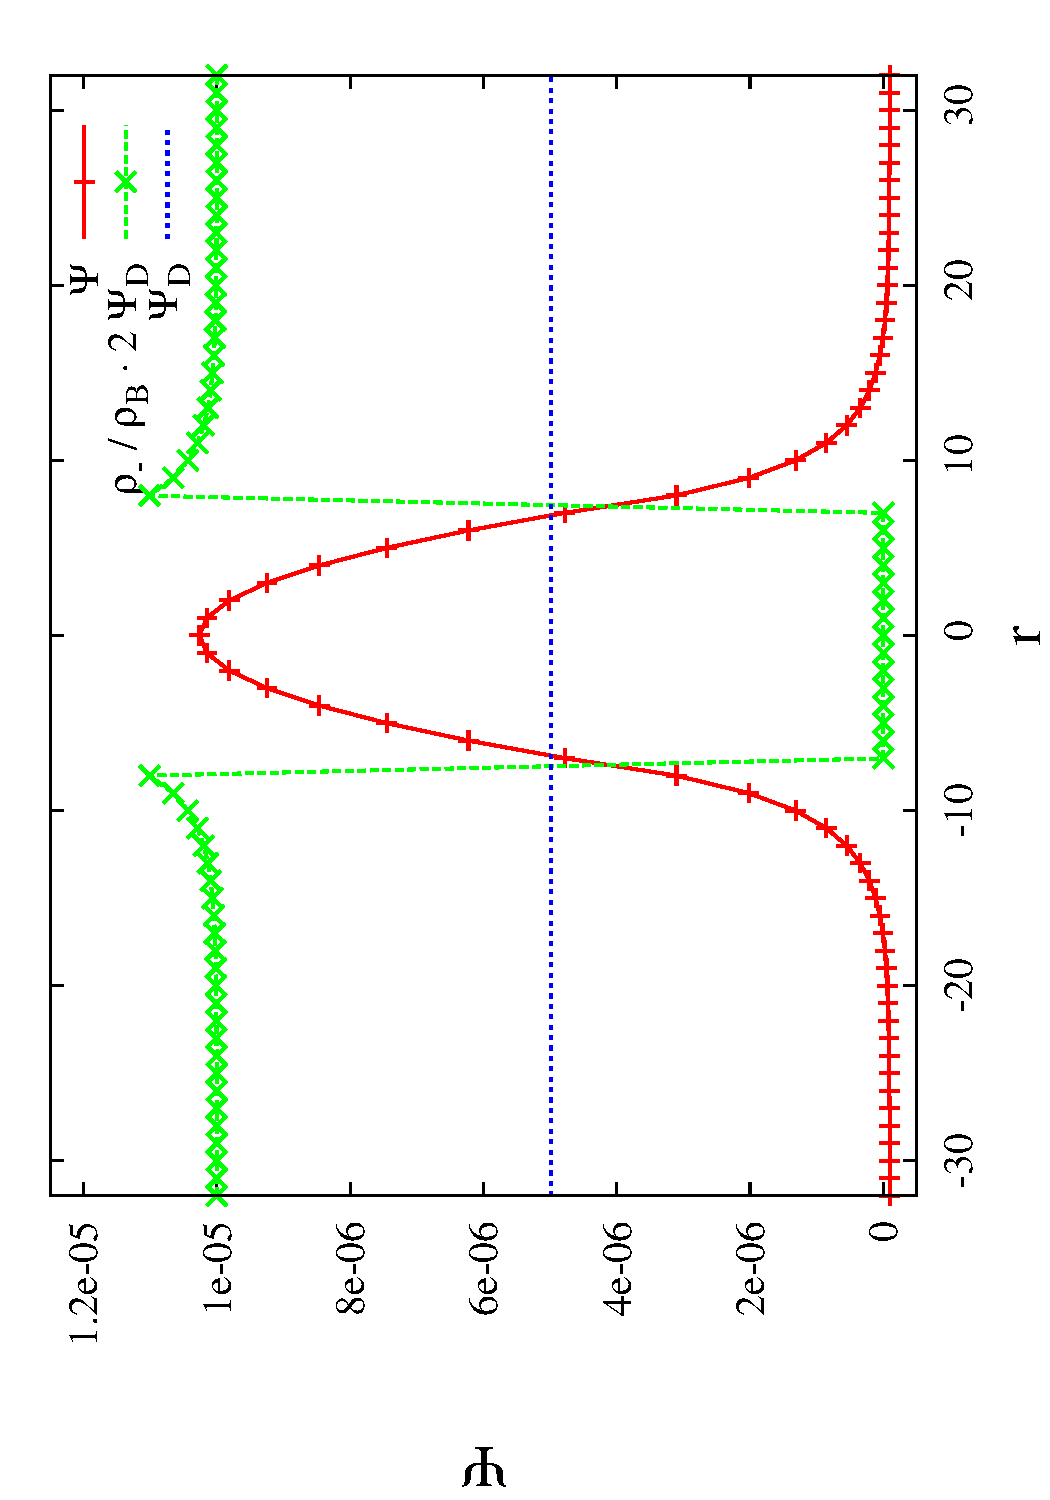
\includegraphics[angle=-90,width=0.9\textwidth]{test_dh2.pdf}
\caption{Debye-H\"uckel theory for positively charged colloid: the picture
shows a cut through the center of a single colloid in a peridoic system.
The potential is shown in red, the Stern potential in blue, and the negative 
charge density in green. The colloid is in the center.}
\label{fig7}
\end{figure}

\clearpage
\begin{thebibliography}{99}

\bibitem{Lyklema} J. Lyklema {\em Fundamentals of Interface and Colloid Science} Academic Press (1995).
\bibitem{Mafe} S. Maf\'e, J.A. Manzanares, J. Pellicer, {\em J. Electroanal. Chem.} {\bf 241}, 57-77 (1988).
\bibitem{Capuani} F. Capuani, I. Pagonabarraga, D. Frenkel, {\em J. Chem. Phys.} {\bf 121}, 973-986 (2004).
\bibitem{Rotenberg} B. Rotenberg, I. Pagonabarraga, D. Frenkel, {\em Farad. Discuss.} {\bf 144}, 223-243 (2010).

\end{thebibliography}

\end{document}


